\chapter{Supplemental material for \chapref{chap:prism}}
\label{chap:prismSuppl}

\begin{figure}[htbp]
\centering
\begin{tabular}{l}
\epsfig{file=figures/prismFigS1.png,width=0.99\linewidth,clip=,trim=0 0 0 0} \\
\end{tabular}
\caption[The addition of species fragments a multiple alignment] {
{\bf The addition of species fragments a multiple alignment.}
{\bf (A)} The multiple alignment format (MAF) represents a multiple alignment as a sequence of alignment blocks. A new block
begins whenever a species is added to or dropped from the aligning sequence. In this example, a single human-rhesus alignment
block is broken into three by the addition of aligning sequence from mouse.
{\bf (B)} For human-based alignments from UCSC, the number of alignment blocks increases and average block length decreases as
more species are included.  Shorter alignment blocks often fragment binding sites (\figref{fig:prismFigS2}), leading to missed
predictions in standard approaches (\figref{fig:prismFigS3}).
}
\label{fig:prismFigS1}
\end{figure}

\begin{figure}[htbp]
\centering
\begin{tabular}{l}
\epsfig{file=figures/prismFigS2.png,width=0.99\linewidth,clip=,trim=0 0 0 0} \\
\end{tabular}
\caption[The PRISM binding site prediction method is robust to challenging technicalities in multiple alignments] {
{\bf The PRISM binding site prediction method is robust to challenging technicalities in multiple alignments.}
{\bf (A)} Conservation-based methods that work exclusively within alignment blocks ignore binding sites that span blocks.
Our approach is robust to fragmentation (see Methods in \ref{sec:prismMethods}).
{\bf (B)} Conceptually, the distance between a binding site in an aligning species and the reference is independent
of other species.  Yet, insertions in third-party species add gap columns to a multiple alignment and exaggerate
local misalignments in alignment space.  To overcome the effect of third-party species, we measure the length of a
shift in genomic coordinates rather than alignment coordinates.
}
\label{fig:prismFigS2}
\end{figure}

\begin{figure}[htbp]
\centering
\begin{tabular}{l}
\epsfig{file=figures/prismFigS3.png,width=0.7\linewidth,clip=,trim=0 0 0 0} \\
\end{tabular}
\caption[Robust PRISM binding site prediction preserves confirmed binding sites] {
{\bf Robust PRISM binding site prediction preserves confirmed binding sites.}
The fraction of binding site predictions confirmed by overlap with a ChIP-seq peak that would be lost due to
multiple alignment issues without our robust implementation would reach 30\% for an expected alignment of 100
mammals (linear extrapolation).  Predictions are summed over the 47 analyzed ENCODE ChIP-seq sets (\tabref{tab:prismTableS2}).
}
\label{fig:prismFigS3}
\end{figure}

\begin{figure}[htbp]
\centering
\begin{tabular}{l}
\epsfig{file=figures/prismFigS4.png,width=0.99\linewidth,clip=,trim=0 0 0 0} \\
\end{tabular}
\caption[Optimizing the run time of binding site prediction] {
{\bf Optimizing the run time of binding site prediction.}
{\bf (A)} The goal of conserved binding site prediction is to identify binding sites in the reference species
using supporting evidence from alignment to other species.  Shown is an example window from a multiple alignment
with a single motif match in the human sequence.  It is only necessary to search for matches to the motif in the
aligning species for a relatively small window around the reference match, with the illustration allowing a
shift of the start position of up to 10 basepairs.
{\bf (B)} PRISM allows a shift size of 20 basepairs, for which the optimization eliminates 90.4\% of the
computation in related species across all motifs.  The variation across motifs reflects how frequently each
motif matches in the human genome.  Whiskers denote 1.5 interquartile distances beyond the upper and lower quartiles.
{\bf (C)} The optimization results in a much reduced runtime to generate the full set of PRISM results and
makes it practical to investigate a larger set of motifs.
}
\label{fig:prismFigS4}
\end{figure}

\begin{figure}[htbp]
\centering
\begin{tabular}{l}
\epsfig{file=figures/prismFigS5.png,width=0.99\linewidth,clip=,trim=0 0 0 0} \\
\end{tabular}
\caption[Transcription factor motifs span a four-fold range of information content specificities] {
{\bf Transcription factor motifs span a four-fold range of information content specificities.}
The motifs in our transcription factor motif library (Fig. 2A) display a broad range of specificities
as measured by information content, which the excess conservation score implicitly considers, typically
requiring deeper conservation for more degenerate motifs (\figref{fig:prismFigS8}).
}
\label{fig:prismFigS5}
\end{figure}

\begin{figure}[htbp]
\centering
\begin{tabular}{l}
\epsfig{file=figures/prismFigS6.png,width=0.50\linewidth,clip=,trim=0 0 0 0} \\
\end{tabular}
\caption[Shuffled motifs serve as a null model] {
{\bf Shuffled motifs serve as a null model.}
We generated shuffled motifs by permuting motif columns while preserving critical properties (see Methods in \ref{sec:prismMethods}).
Shown are the GLI2 motif and example rejected and accepted shuffles.
}
\label{fig:prismFigS6}
\end{figure}

\begin{figure}[htbp]
\centering
\begin{tabular}{l}
\epsfig{file=figures/prismFigS7.png,width=0.99\linewidth,clip=,trim=0 0 0 0} \\
\end{tabular}
\caption[Number of shuffled motifs per transcription factor motif] {
{\bf Number of shuffled motifs per transcription factor motif.}
{\bf (A)} We attempted to create ten shuffled versions of each transcription factor motif (\figref{fig:prismFigS6}).
Most motifs (249 of 332; 75\%) produce a complete set of ten shuffles.
{\bf (B)} For some motifs, such as HOXA1, it is not possible to generate ten unique shuffles due to degeneracy in the motif.
}
\label{fig:prismFigS7}
\end{figure}

\begin{figure}[htbp]
\centering
\begin{tabular}{l}
\epsfig{file=figures/prismFigS8.png,width=0.99\linewidth,clip=,trim=0 0 0 0} \\
\end{tabular}
\caption[Excess conservation score measures the statistical significance of binding site conservation, accounting
for genomic context and motif properties] {
{\bf Excess conservation score measures the statistical significance of binding site conservation, accounting
for genomic context and motif properties.}
{\bf (A)} Excess conservation score as a function of Bayesian branch length (motif score) for NFYA across five
different \% identify bins (see Methods in \ref{sec:prismMethods}).  A given depth of conservation, as measured by Bayesian branch length,
is more impressive, and thus produces a higher excess conservation score in less conserved neighborhoods than in
highly conserved neighborhoods (also see~\figref{fig:prismFig1}C).
{\bf (B)} Excess conservation as a function of Bayesian branch length (motif score) for REST, IRF5, and CEBPA
in the 70\% identity region.  A given depth of conservation is more impressive for a stronger motif, such as REST,
than for a weaker motif, such as CEBPA (see~\figref{fig:prismFigS5}), as the weak motif is more tolerant of
substitutions and spurious conserved hits are more likely.
}
\label{fig:prismFigS8}
\end{figure}

\begin{figure}[htbp]
\centering
\begin{tabular}{l}
\epsfig{file=figures/prismFigS9.png,width=0.90\linewidth,clip=,trim=0 0 0 0} \\
\end{tabular}
\caption[Most biological context terms are not falsely enriched for shuffled motifs] {
{\bf Most biological context terms are not falsely enriched for shuffled motifs.}
{\bf (A)} For the human genome, the vast majority of terms -- 21,901 of the 27,956 (78\%) -- are not significant
for any of the 2,857 shuffled motifs that we analyzed.  We retained only enrichments for terms with an Expected
value $\leq 1$ (see Methods in \ref{sec:prismMethods}), which is satisfied by a full 25,466 (91\%) terms.
{\bf (B)} The results are similar for the mouse genome: 19,904 of the 26,656 terms (75\%) are not significant for
any shuffled motif, and we retain 23,310 (87\%) of terms at an Expected value $\leq 1$.
}
\label{fig:prismFigS9}
\end{figure}

\begin{figure}[htbp]
\centering
\begin{tabular}{l}
\epsfig{file=figures/prismFigS10.png,width=0.50\linewidth,clip=,trim=0 0 0 0} \\
\end{tabular}
\caption[Diversity of PRISM predictions in the human genome] {
{\bf Diversity of PRISM predictions in the human genome.}
For human, PRISM's 1,658 predicted associations between a transcription factor and a biological role derive
from 9 different ontologies that cover a variety of topics, at a false discovery rate of 14.8\%.
}
\label{fig:prismFigS10}
\end{figure}

\begin{figure}[htbp]
\centering
\begin{tabular}{l}
\epsfig{file=figures/prismFigS11.png,width=0.99\linewidth,clip=,trim=0 0 0 0} \\
\end{tabular}
\caption[Diversity of PRISM predictions in the mouse genome] {
{\bf Diversity of PRISM predictions in the mouse genome.}
For mouse, PRISM's 1,173 predicted associations between a transcription factor and a biological role
{\bf (A)} cover most major DNA binding domain families, and
{\bf (B)} derive from 8 different ontologies, at a false discovery rate of 16.1\%.
}
\label{fig:prismFigS11}
\end{figure}

\begin{figure}[htbp]
\centering
\begin{tabular}{l}
\epsfig{file=figures/prismFigS12.png,width=0.99\linewidth,clip=,trim=0 0 0 0} \\
\end{tabular}
\caption[PRISM function associations are supported by dozens to hundreds of binding site and gene targets] {
{\bf PRISM function associations are supported by dozens to hundreds of binding site and gene targets.}
{\bf (A)} Number of binding site and gene targets that support each of the 1,658 PRISM transcription factor role predictions for human.
{\bf (B)} Number of binding site and gene targets that support each of the 1,173 PRISM transcription factor role predictions for mouse.
}
\label{fig:prismFigS12}
\end{figure}

\FloatBarrier

\begin{table}[htbp]
\begin{center}
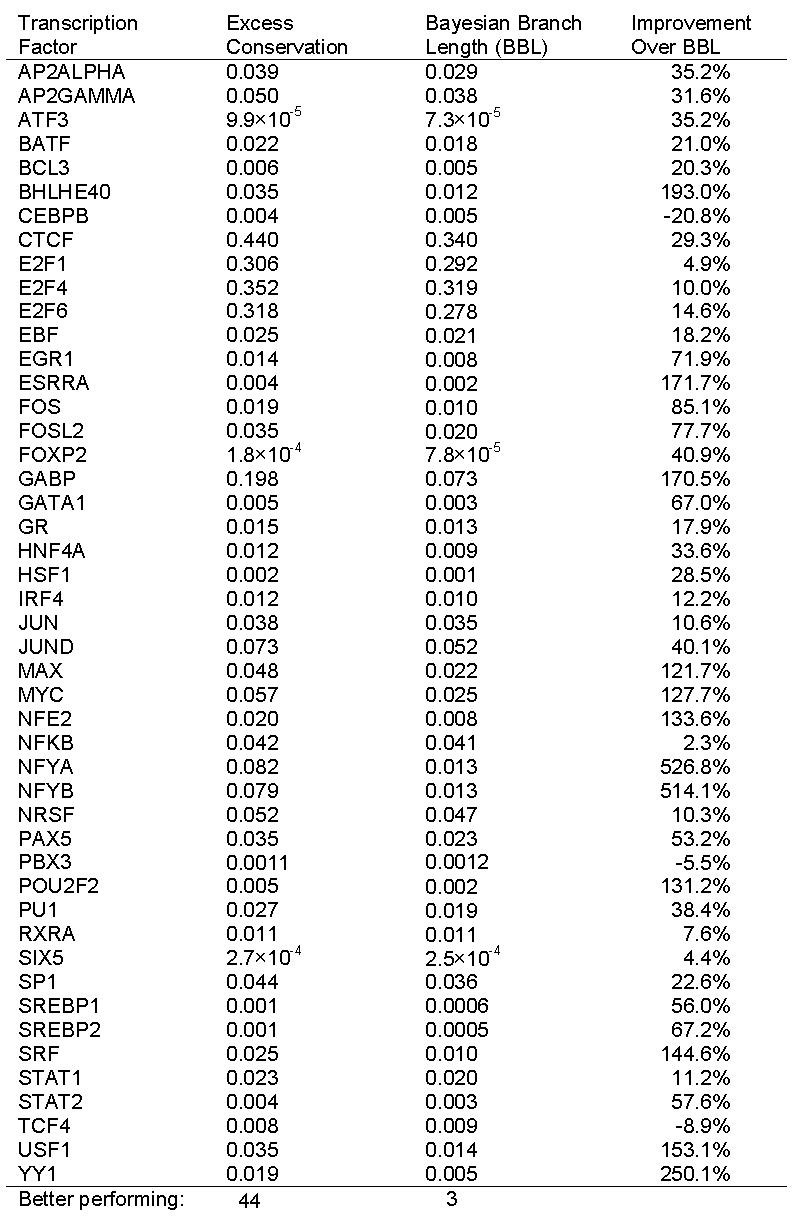
\includegraphics[width=0.8\linewidth]{figures/prismTableS1.pdf}
\caption[Excess conservation improves binding site prediction]{
{\bf Excess conservation improves binding site prediction.}
Shown is the area under the Precision-Recall curve for binding site prediction with and without
excess conservation adjustment, as measured by overlap of binding site predictions with ChIP-seq
peaks (\tabref{tab:prismTableS2}).
}
\label{tab:prismTableS1}
\end{center}
\end{table}

\begin{table}[htbp]
\begin{center}
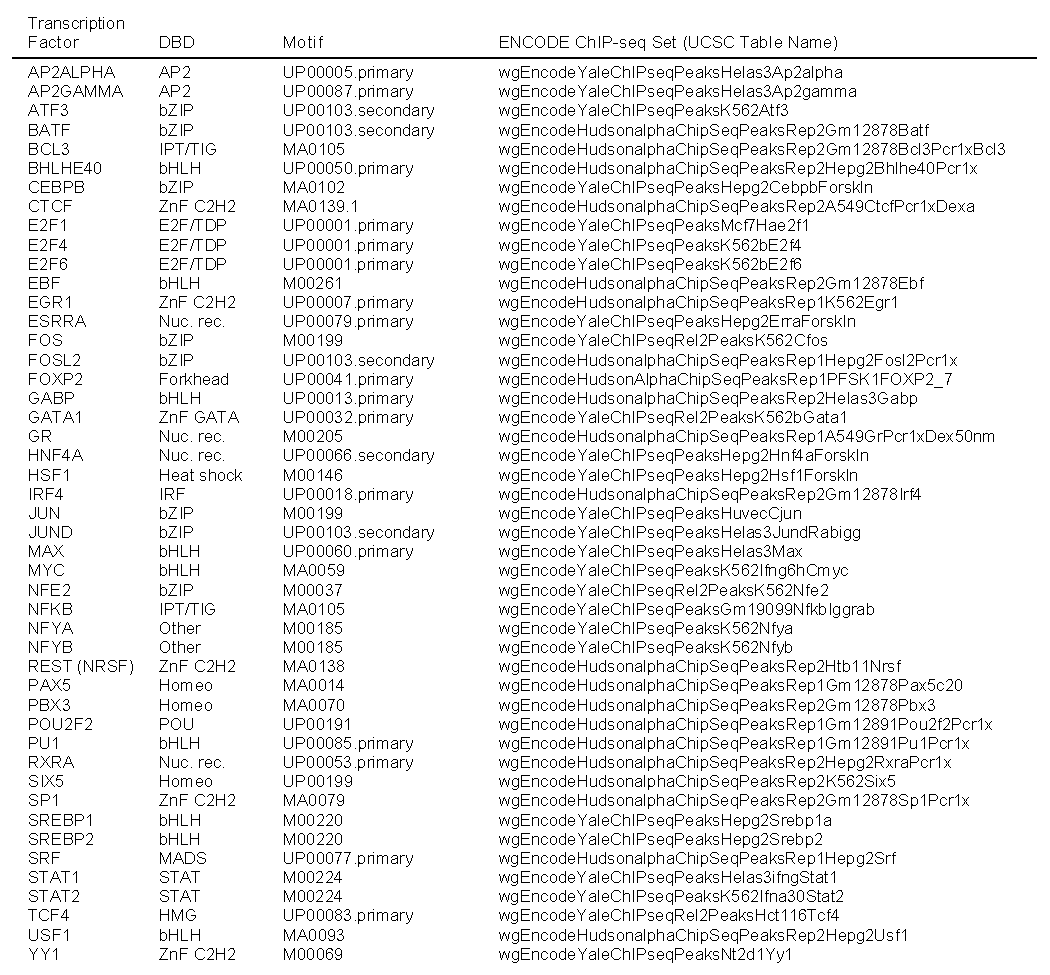
\includegraphics[width=0.99\linewidth]{figures/prismTableS2.pdf}
\caption[Motifs used for comparison with ChIP-seq]{
{\bf Motifs used for comparison with ChIP-seq.}
We compared binding site predictions using transcription factor motifs to the largest ChIP-seq data set from the ENCODE
Consortium~\citep{Encode2011} for 47 transcription factors. For motifs, ``UP'' specifies UniPROBE~\citep{Newburger2009},
``MA'' specifies JASPAR~\citep{Bryne2008}, and ``M'' specifies TransFac~\citep{Matys2006}. ``DBD'' DNA binding domain.
}
\label{tab:prismTableS2}
\end{center}
\end{table}

\begin{table}[htbp]
\begin{center}
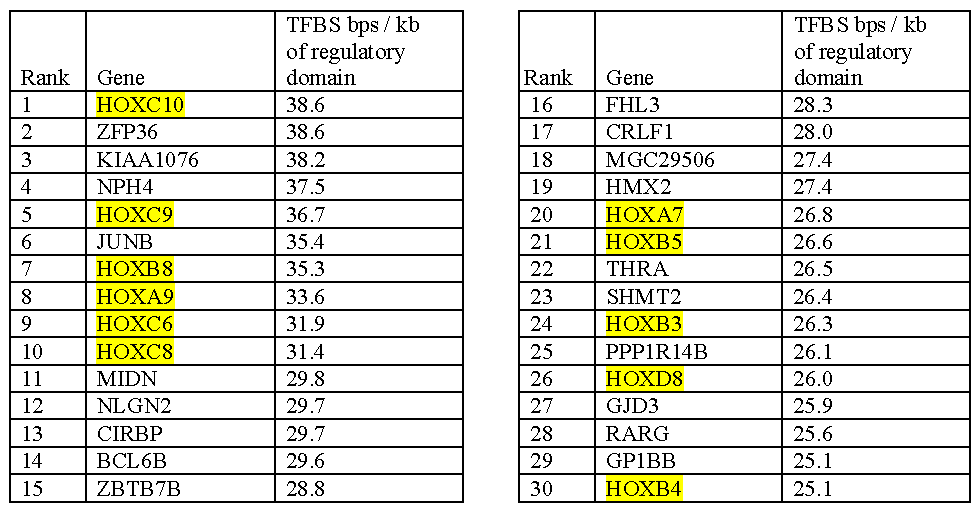
\includegraphics[width=0.99\linewidth]{figures/prismTableS3.pdf}
\caption[The HOX genes are among the most densely regulated human genes]{
{\bf The HOX genes are among the most densely regulated human genes.}
Eleven of the top 30 human genes by density of PRISM binding site predictions are HOX genes, with representatives
from all four HOX clusters.  Predicted binding sites are combined for all 332 motifs in the PRISM motif library,
and only genes with predicted regulatory domains over 10kb are considered.  TFBS: transcription factor binding
sites; bps: basepairs; kb: 1,000 basepairs.  Yellow highlighting: HOX gene.
}
\label{tab:prismTableS3}
\end{center}
\end{table}

\begin{table}[htbp]
\begin{center}
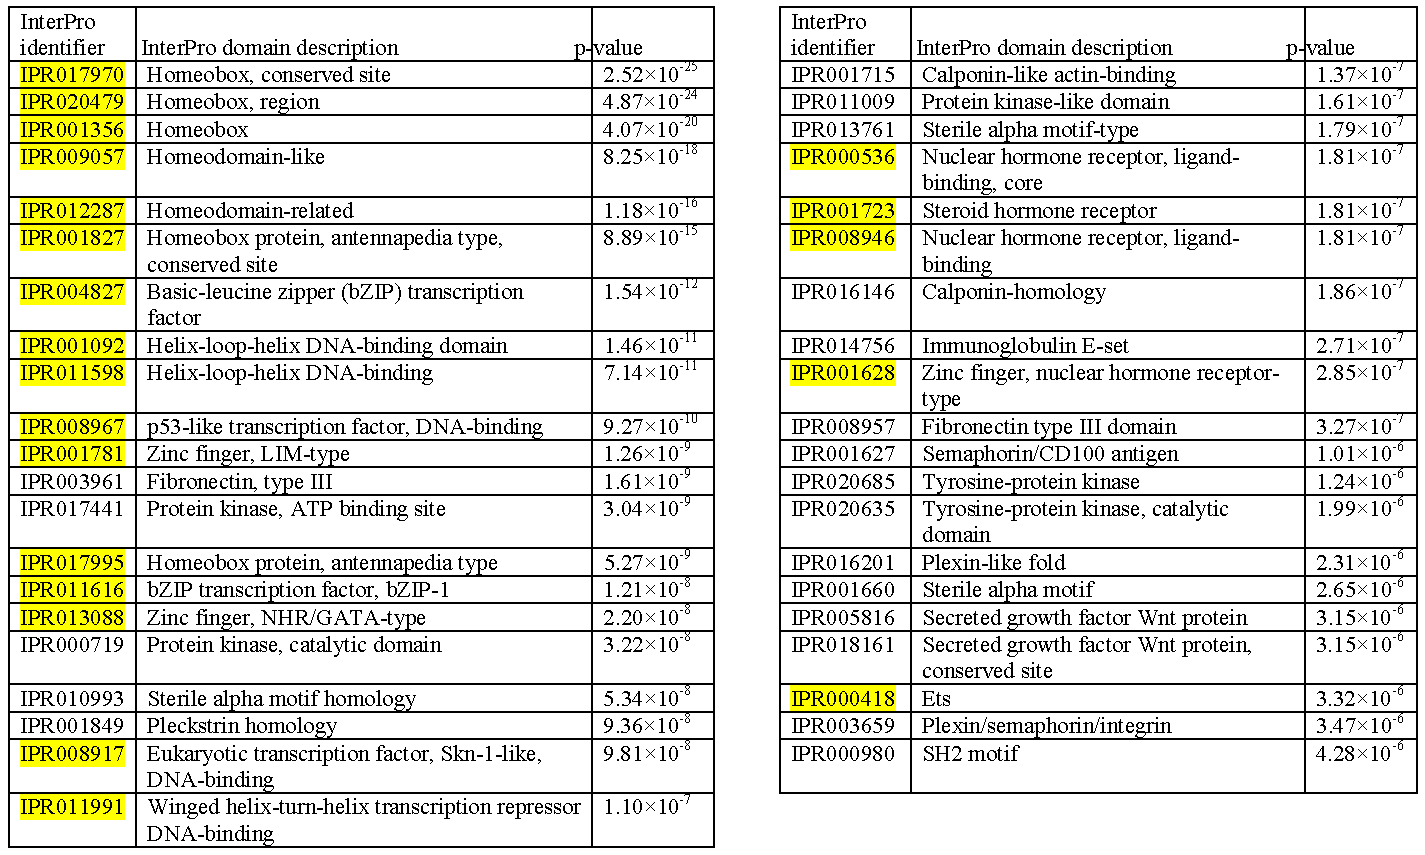
\includegraphics[width=0.99\linewidth]{figures/prismTableS4.pdf}
\caption[Transcription factor gene families are highly regulated]{
{\bf Transcription factor gene families are highly regulated.}
Many of the InterPro~\citep{Hunter2009} domains with the densest upstream regulation are transcription factor
domains.  Individual human genes were ranked by the fraction of basepairs in the gene regulatory domain that
include a PRISM binding site prediction.  For each InterPro term, a Wilcoxon rank-sum test was used to determine
whether the genes with the term have surprisingly dense regulatory domains.  All significant
families (Bonferroni corrected p-value $<$ 0.05) are shown.  Yellow highlighting: transcription factor DNA binding domain.
}
\label{tab:prismTableS4}
\end{center}
\end{table}

\begin{table}[htbp]
\begin{center}
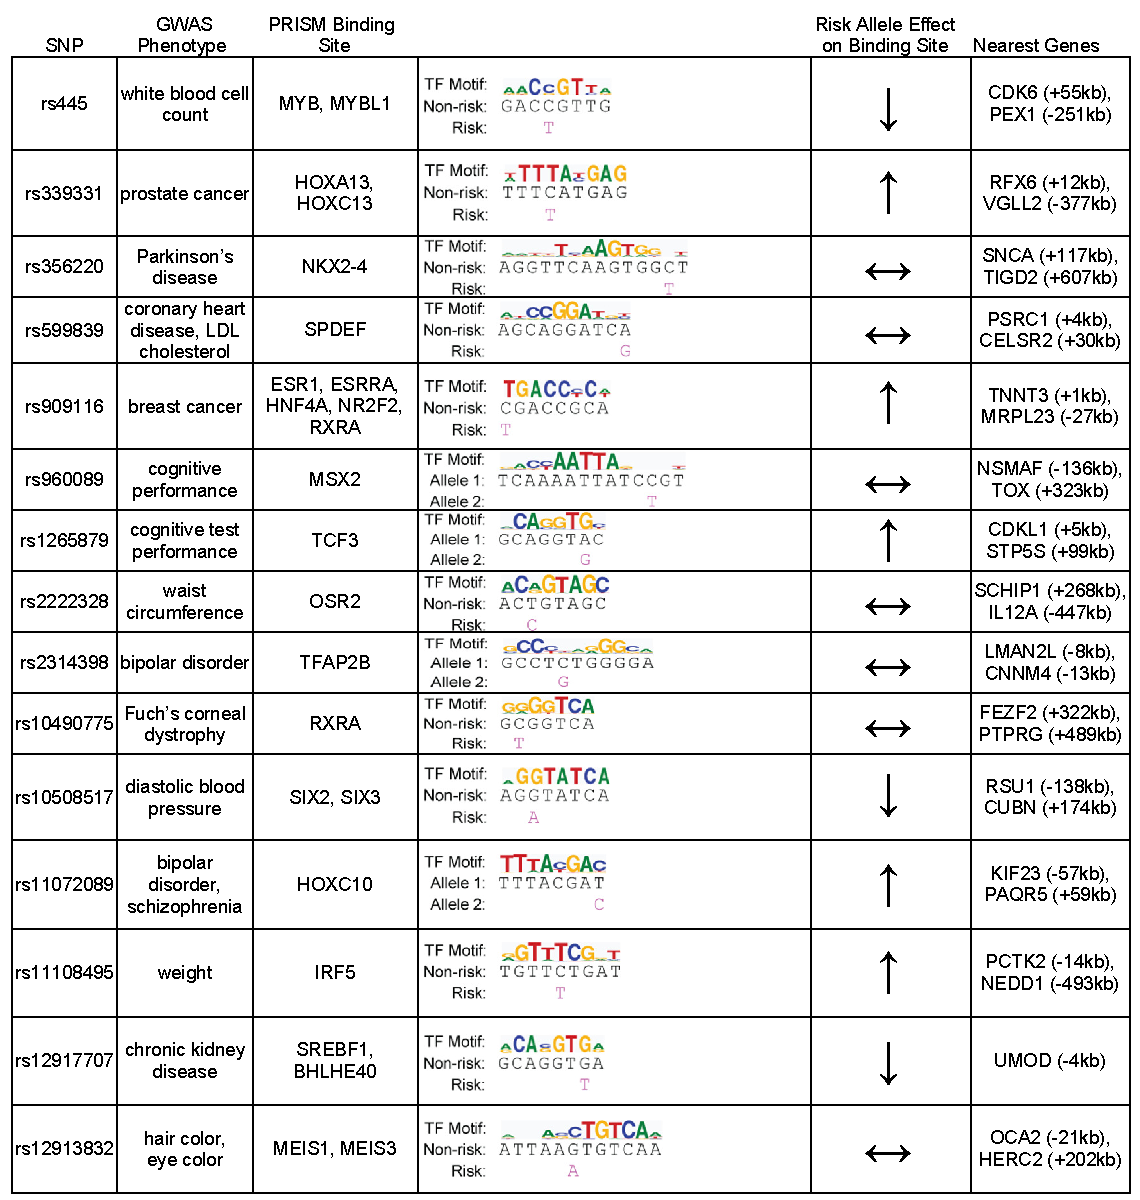
\includegraphics[width=0.99\linewidth]{figures/prismTableS5.pdf}
\caption[PRISM identifies conserved binding sites that overlap 15 GWAS phenotype-associated SNPs]{
{\bf PRISM identifies conserved binding sites that overlap 15 GWAS phenotype-associated SNPs.}
PRISM identifies potentially causative binding sites affected by phenotype-associated SNPs.
The risk allele either disrupts (down arrow), introduces (up arrow), or has little effect
(horizontal arrow) on the predicted binding site.
}
\label{tab:prismTableS5}
\end{center}
\end{table}

\begin{table}[htbp]
\begin{center}
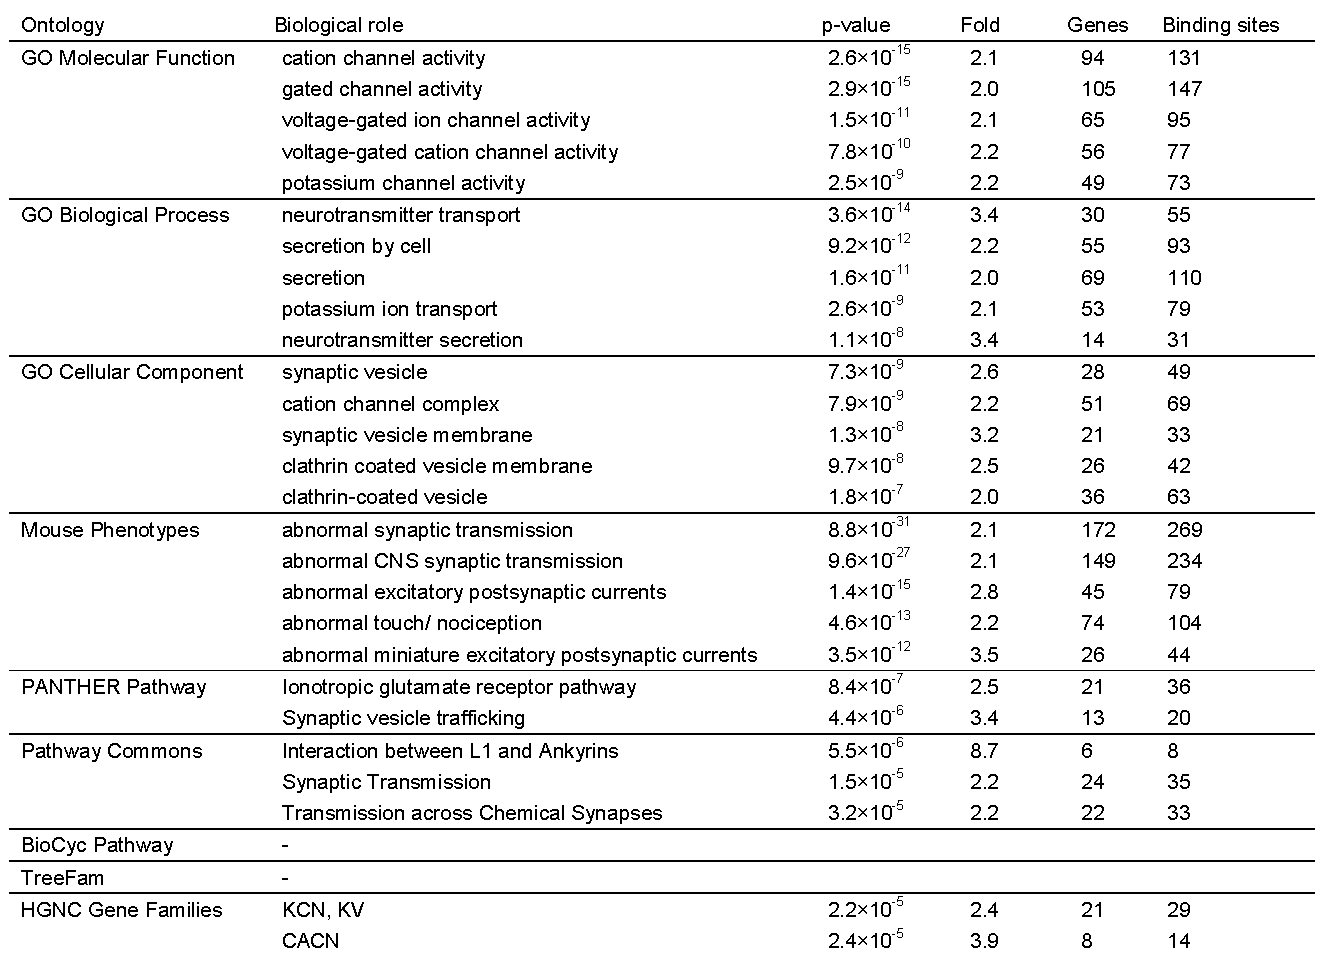
\includegraphics[width=0.99\linewidth]{figures/prismTableS6.pdf}
\caption[GREAT enrichments for REST ChIP-seq binding sites]{
{\bf GREAT enrichments for REST ChIP-seq binding sites.}
Shown are the biological role enrichments that satisfy GREAT default statistical significant thresholds for
1,712 REST ChIP-seq binding sites from human Jurkat T cells~\citep{Valouev2008}.  At most five significant
results are shown per ontology.
}
\label{tab:prismTableS6}
\end{center}
\end{table}

\begin{table}[htbp]
\begin{center}
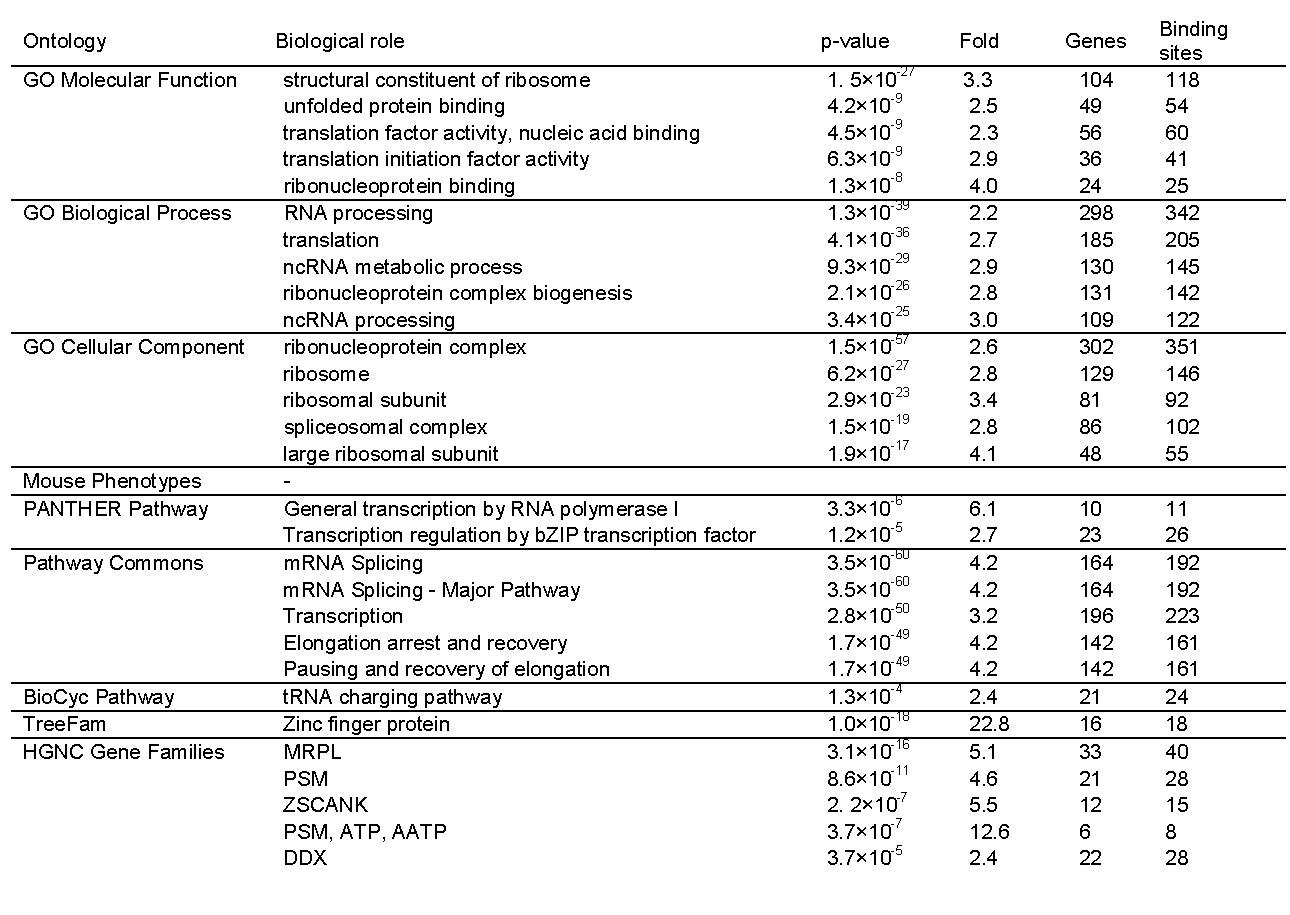
\includegraphics[width=0.99\linewidth]{figures/prismTableS7.pdf}
\caption[GREAT enrichments for GABPA ChIP-seq binding sites]{
{\bf GREAT enrichments for GABPA ChIP-seq binding sites.}
Shown are the biological role enrichments that satisfy GREAT default statistical significant thresholds
for 3,585 \textit{GABPA} ChIP-seq binding sites from human Jurkat T cells~\citep{Valouev2008}.  At most five
significant results are shown per ontology.
}
\label{tab:prismTableS7}
\end{center}
\end{table}

\begin{table}[htbp]
\begin{center}
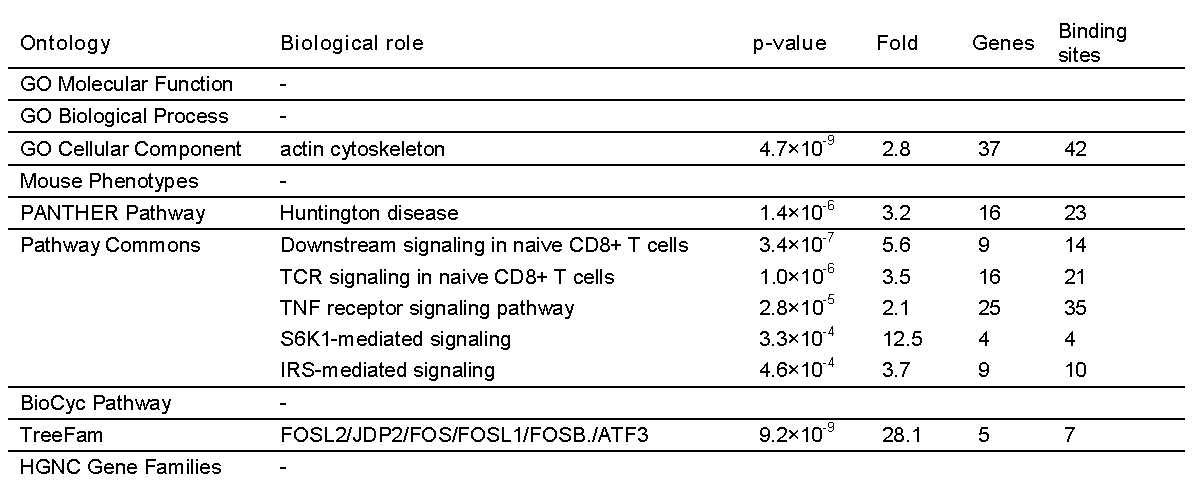
\includegraphics[width=0.99\linewidth]{figures/prismTableS8.pdf}
\caption[GREAT enrichments for SRF ChIP-seq binding sites]{
{\bf GREAT enrichments for SRF ChIP-seq binding sites.}
Shown are the biological role enrichments that satisfy GREAT default statistical significant thresholds for
556 SRF ChIP-seq binding sites from human Jurkat T cells~\citep{Valouev2008}.  At most five significant
results are shown per ontology.
}
\label{tab:prismTableS8}
\end{center}
\end{table}

\begin{table}[htbp]
\begin{center}
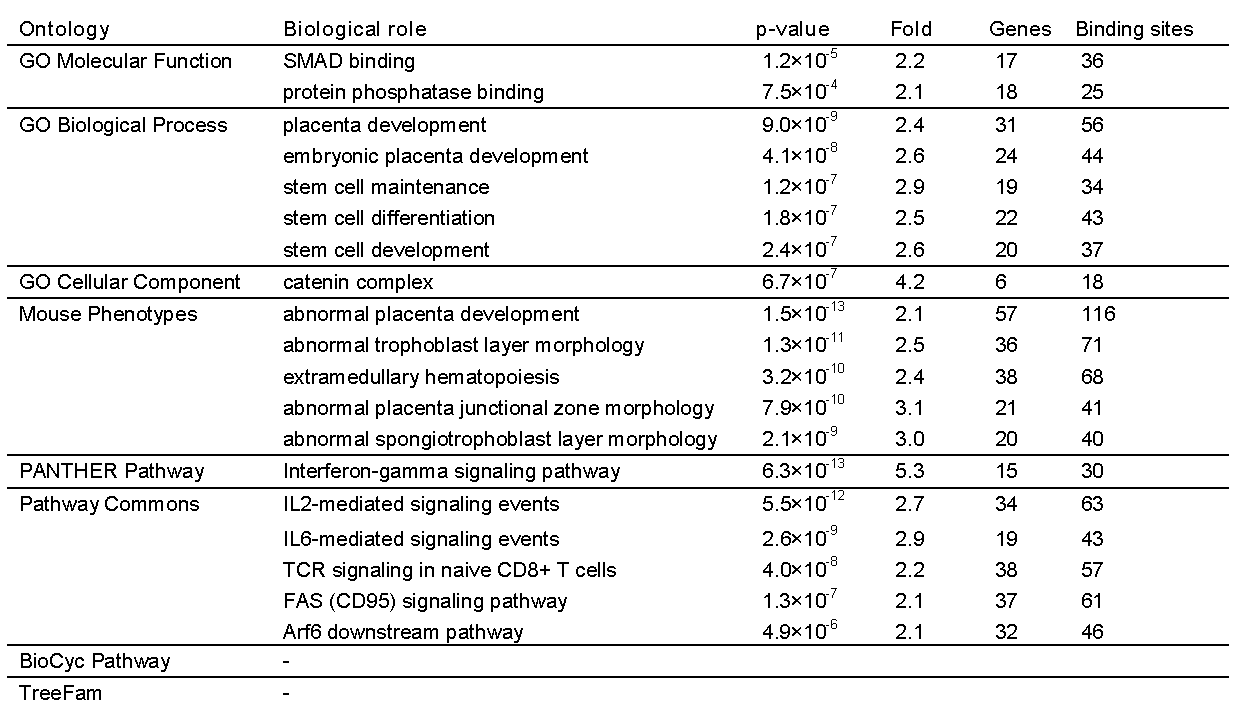
\includegraphics[width=0.99\linewidth]{figures/prismTableS9.pdf}
\caption[GREAT enrichments for Stat3 ChIP-seq binding sites]{
{\bf GREAT enrichments for Stat3 ChIP-seq binding sites.}
Shown are the biological role enrichments that satisfy GREAT default statistical significant thresholds for
1,568 Stat3 ChIP-seq binding sites from mouse embryonic stem cells~\citep{Chen2008}.  At most five significant
results are shown per ontology.
}
\label{tab:prismTableS9}
\end{center}
\end{table}

\begin{table}[htbp]
\begin{center}
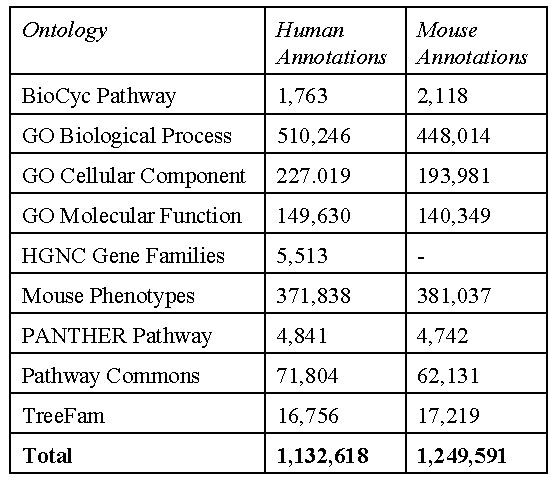
\includegraphics[width=0.45\linewidth]{figures/prismTableS10.pdf}
\caption[GREAT ontologies used by PRISM]{
{\bf GREAT ontologies used by PRISM.}
Annotations is the number of distinct term-to-gene pairs in the ontology.
}
\label{tab:prismTableS10}
\end{center}
\end{table}

\begin{table}[htbp]
\begin{center}
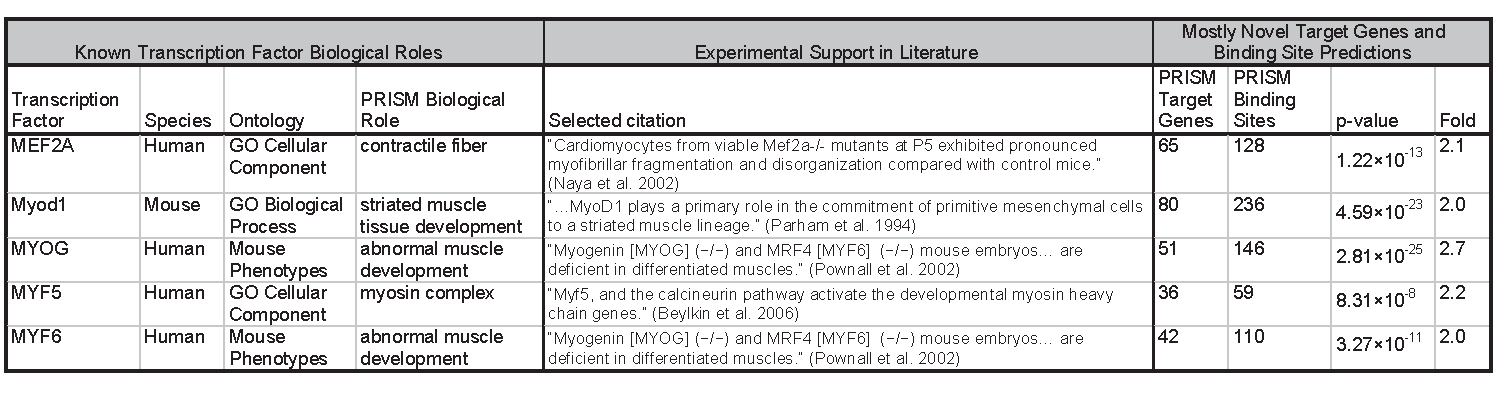
\includegraphics[width=0.99\linewidth]{figures/prismTableS13.pdf}
\caption[PRISM offers excellent depth of coverage for the muscle differentiation network and highlights nuanced functions of key factors]{
{\bf PRISM offers excellent depth of coverage for the muscle differentiation network and highlights nuanced functions of key factors.}
Shown is the top muscle related term and citation of experimental support for each of five main regulators of muscle differentiation.
PRISM extends current knowledge of the muscle differentiation network by identifying many novel relevant target genes and binding
sites for each transcription factor.
}
\label{tab:prismTableS13}
\end{center}
\end{table}
